\chapter{Methodology}
Our primary goal is to achieve the swing-up movement in the pendubot or acrobot setup and to maintain stability around the highest points. Initial training trials with reinforcement learning have revealed challenges. These include potential entrapment in local minima and difficulty in maintaining stability at the highest point for extended periods. 

To address these challenges, we adopt two main strategies. For the stabilization issue, we introduce a combined controller. During the swing-up process, an RL-trained agent, using the Soft Actor-Critic—a classic model-free reinforcement learning algorithm—assumes control based on its learned policies. Yet, as the system nears the maximum point, a seamless transition takes place. This shift allows a continuous-time LQR controller to take over, ensuring the final stabilization required to maintain stability at the highest point.

\section{Soft actor critic}
Within the landscape of reinforcement learning, the Soft Actor Critic (SAC)\cite{haarnoja2018soft} stands out as an algorithm specifically designed for environments with continuous state and action spaces. Such environments, exemplified by our double pendulum system where actuators can be adjusted to any value within the torque limit range, and state measurement can take any real number, influenced our decision to adopt SAC.

Like many other deep reinforcement learning algorithms, SAC optimizes a policy by maximizing the expected cumulative reward the agent obtains over time. This optimization is primarily achieved through an actor-critic structure\cite{konda1999actor}.

The actor determines the best actions by interpreting the current environmental conditions and adhering to the existing policy. Typically, the actor is visualized as a shallow neural network that approximates the mapping between the input state and the output probability distribution over actions. Furthermore, SAC incorporates a stochastic policy within its actor, which fosters exploration and aids the agent in refining its policies.

On the other hand, the critic evaluates the value of state-action pairs. It estimates the expected cumulative reward the agent can achieve by following a particular policy. More often than not, the critic is depicted as a neural network that processes state-action pairs as inputs to yield the estimated value.

A distinguishing feature of SAC, besides the actor-critic framework, is entropy regularization\cite{achiam2018spinning}. SAC utilizes a stochastic policy. This means that instead of always settling on a single best action for each state, the agent considers a probability distribution over potential actions. The incorporation of entropy in SAC aims to encourage exploration: high entropy signifies a more uniform distribution, implying the agent's uncertainty and tendency to explore diverse actions, while low entropy points to a concentrated distribution, suggesting the agent's confidence in a specific action. By definition, entropy quantifies randomness. Within SAC, it captures the unpredictability of the policy's action distribution. If
\(x\) is a random variable with a probability density function \(P\), the
entropy \(H\) of \(x\) is defined as:

\begin{equation}
 H(P) = \displaystyle \mathop{\mathbb{E}}_{x \sim P}[-\log P(x)]
\end{equation}

By maximizing entropy, SAC encourages exploration and accelerates learning. It
also prevents the policy from prematurely converging to a suboptimal solution.
The trade-off between maximizing reward and maximizing entropy is controlled
through a parameter, \(\alpha\). This parameter serves to balance the importance
of exploration and exploitation within the optimization problem. The optimal policy
\(\pi^*\) can be defined as follows:

\begin{equation}
 \pi^* = {arg}{\max_{\pi}}{\displaystyle
 \mathop{\mathbb{E}}_{\tau\sim\pi}}{\Bigg[{\sum_{t=0}^{\infty}}{\gamma^{t}}{\Big(R(s_t,a_t,s_{t+1})}+{\alpha}H(\pi(\cdot\mid{s_t}))\Big)\Bigg]}
\end{equation}

During training, SAC learns a policy $\pi_{\theta}$ and two Q-functions
$Q_{\phi_1} , Q_{\phi_2}$ concurrently. The loss functions for the two Q-networks are
$(i \in {1, 2})$:

\begin{equation}
  L(\phi_i,D) = \displaystyle
  \mathop{\mathbb{E}}_{(s,a,r,s',d)\sim{D}}\bigg[\bigg(Q_{\phi_i}(s,a)-y(r,s',d)\bigg)^2\bigg],
\end{equation}

where the temporal difference target \(y\) is given by:
\begin{align}
  y(r,s',d) &= r + \gamma(1-d) \times \nonumber\bigg(\displaystyle
  \mathop{\min}_{j=1,2}Q_{\phi_{targ,j}}(s',\tilde{a}')-\alpha\log
  {\pi_\theta}(\tilde{a}'\mid{s}')\bigg), \\
  \tilde{a}'&\sim{\pi_\theta}(\cdot\mid{s'})
\end{align}

In each state, the policy \(\pi_\theta\) should act to maximize the expected
future return \(Q\) while also considering the expected future entropy \(H\). In other
words, it should maximize \(V^\pi(s)\):
\begin{align}
 V^\pi(s) &= {\displaystyle \mathop{\mathbb{E}}_{a\sim\pi}[Q^\pi(s,a)]} +
 \alpha{H(\pi(\cdot\mid{s}))} \\
 &= {\displaystyle \mathop{\mathbb{E}}_{a\sim\pi}[Q^\pi(s,a)]} -
 \alpha{\log {\pi(a\mid{s})}}
\end{align}


By employing an effective gradient-based optimization technique, the parameters
of both the actor and critic neural networks undergo updates, subsequently
leading to the adaptation of the policies themselves.

In conclusion, SAC's combination of stochastic policies, exploration through
entropy regularization, value estimation, and gradient-based optimization make
it a well-suited algorithm for addressing the challenges posed by continuous
state and action spaces.

\section{Linear quadratic regulator}
The Linear Quadratic Regulator (LQR)\cite{lehtomaki1981robustness} is an effective control method primarily designed for linear systems. Yet, when dealing with nonlinear dynamics, it remains applicable.The nonlinear system is linearized around a selected operating point, and based on this linearized version, the LQR controller can be sculpted.

Taking a step back, the general form of a nonlinear system can be expressed as:
\begin{equation}
 \dot{x}(t) = f(x(t), u(t))
\end{equation}


In certain applications like pendubot or acrobot stabilization, it is important to select the appropriate operating point. We select the operating point around the upright position, specifically \(x_{op} = [\pi,0,0,0]^T\). Around this point, the system can be linearized, leading to:

\begin{equation}
\dot{\overline{x}}(t) = A \overline{x}(t) + B u(t)
\end{equation}


Here, the deviation from the desired state is given by \(\overline{x} = x - x_{\text{op}}\), and its first derivative, \(\dot{\overline{x}} = \dot{x}\). The linearized  matrices \(A\) and \(B\) are derived as:

\begin{equation}
 A = \left.\frac{\partial f}{\partial x}\right|_{\text{op}}, \quad B = \left.\frac{\partial f}{\partial u}\right|_{\text{op}}
\end{equation}


To derive an optimal control strategy, we use a quadratic cost function \(J\):

\begin{equation}
  J = \int_0^{\infty} \left( x^T Q x + u^T R u \right) \, dt
\end{equation}

Usually, the matrices \(Q\) and \(R\) are chosen to be symmetric and positive definite, which means \(Q = Q^T\) and all its eigenvalues are positive, and similarly \(R = R^T\) with all positive eigenvalues. With such choices, the Hamilton-Jacobi-Bellman equation, whose solution gives the optimal cost-to-go function from which the optimal policy is derived, can be reduced to the continuous-time algebraic Riccati equation.

\begin{equation}
 A^T S + SA - SBR^{-1}B^T S + Q = 0
\end{equation}

Finally, the LQR control law obtained with above method for this linearized system is:
\begin{equation}
 u(t) = -K\overline{x}(t)
\end{equation}
with \(K = R^{-1}B^T S\).

For an infinite-horizon LQR controller like this, torques will always be applied to steer the system state toward the origin of the linear system.


\section{Combining SAC and LQR with region of attraction}
In our approach, we employ a combined control method for both the swing-up and stabilization tasks. During the swing-up phase, we utilize the SAC controller. Once the state of the double pendulum approaches the vicinity of the desired goal state, we transition from the SAC controller to the LQR controller for final-stage stabilization. A vital aspect of any combined control strategy is determining the conditions under which the system is primed for a transition between control methods. In our SAC+LQR control strategy, the region of attraction method\cite{maywald2022co} serves as the criterion for making this determination.

The region of attraction (ROA) for a nonlinear system, represented by \(R_a\), signifies the set \(\mathcal{B}\) of initial states surrounding a fixed point \(x_0\). If a state lies within this region, the system will gravitate towards \(x_0\) as \(t \rightarrow \infty\). In the context of an LQR controller, the ROA demarcates the area within the state space where the controlled system exhibits asymptotic stability. For complex systems, directly computing \(R_a\) can be challenging; it is often estimated instead. Therefore, analyzing the stability of the controlled system within this region becomes crucial. The state space representation of a controlled linear system can be expressed as:

\begin{equation}
\dot{x}(t) = (A - BK)x(t)
\end{equation}

where \(A_c = A - BK\).

The most straightforward way to analyze the stability of a system is using the Lyapunov method. We choose a Lyapunov function in a quadratic form:
\begin{equation}
  V(\bar{x}) = \bar{x}^T S_{LQR} \bar{x} 
\end{equation}

where \(S_{LQR}\) is a positive definite matrix. This function serves as an "energy-like" metric, and our goal is to demonstrate its decrease over time for a stable system.

Next, we compute the time derivative of the Lyapunov function. For the infinite horizon LQR, \(\frac{\partial S_{LQR}}{\partial t} = 0\) and \(\frac{\partial x_0}{\partial t} = 0\), hence \(\dot{V}\) is:

\begin{equation}
\dot{V}(\overline{x}) = 2\overline{x}^{T}S_{LQR}\dot{\overline{x}}
\end{equation}

For the system to be asymptotically stable at the equilibrium \(x_{op}\), we require the system to satisfy the Lyapunov conditions:

\begin{equation}
\begin{cases}
   V(\overline{x}) > 0 \\
   \dot{V}(\overline{x}) < 0 & \text{for all} \quad x \neq x_{op}
\end{cases}
\end{equation}

To construct an optimizable region of attraction, we define an upper bound \(\rho\) for the Lyapunov function \(V\). We seek the greatest \(\rho\) such that the above Lyapunov conditions are satisfied:

\begin{equation}
\begin{cases}
    \mathcal{B} = \{ x \mid 0 < V(x) < \rho \} \\
    \dot{V}(x) = 2\bar{x}^T S_{LQR} \dot{\bar{x}} < 0
\end{cases}
\end{equation}

We computed the RoA similar to\cite{maywald2022co} but with a sums of squares method\cite{tedrake2010lqr}.  Consequently, the resulting shape of the ROA in a 4D state space resembles an ellipsoid.
\begin{figure}[htbp]
    \centering
    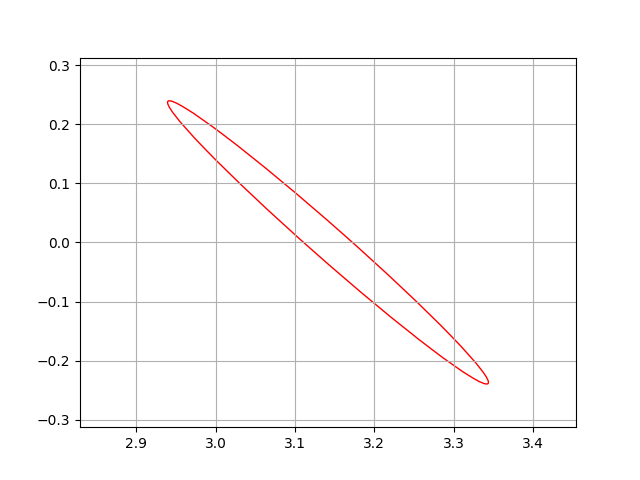
\includegraphics[width=0.6\textwidth]{figures/methodology/roaplot.png} % Adjust the width as needed
    \caption{Region of Attraction}
    \label{fig:example}
\end{figure}

Once the RoA is computed, it can be checked whether a state \(x\) belongs to the estimated RoA of the LQR controller by calculating the cost-to-go of the LQR controller with the matrix \(S_{LQR}\) and comparing it with the scalar \(\rho\).

\section{Reward shaping}
In theory, the reward function is designed to guide the agent's behavior towards achieving stability around the system's goal point. However, initial training attempts have revealed challenges. For instance, the agent might get stuck in a local minimum for an extended period, fail to perform a swing-up, or be unable to maintain stability around the upright position for a prolonged duration. The stabilization problem is addressed by the LQR controller and its region of attraction, which guarantees asymptotic stability. To tackle the swing-up issue, we designed a customized three-stage reward function to steer the agent away from problematic local minima and into the region of attraction of the LQR controller. The full equation for this reward function is:
\begin{equation}
\begin{aligned}
 r(x,u) = &-(x - x_g)^T Q_{train} (x - x_g) - u^T R_{train}u \\
           & +
            \begin{dcases*}
              r_{line} & \text{if} $h(p_1, p_2) \geq h_{line}$\, ,\\
              0 & \text{else}
            \end{dcases*}\\
           & +
            \begin{dcases*}
              r_{LQR} & \text{if} $(x - x_g)^T S_{LQR} (x - x_g) \geq \rho $\, ,\\
              0 & \text{else}
            \end{dcases*}\\
           & -
            \begin{dcases*}
              r_{vel} & \text{if} $|v_1| \geq v_{thresh}$\, ,\\
              0 & \text{else}
            \end{dcases*}\\
           & -
            \begin{dcases*}
              r_{vel} & \text{if} $|v_2| \geq v_{thresh}$\, ,\\
              0 & \text{else}
            \end{dcases*}
\end{aligned}
\end{equation}

In the initial stage, a quadratic reward function is employed to encourage
smooth swinging of the entire system within a relatively small number of
training sessions. The matrix  \(Q_{train} = diag(Q_1, Q_2, Q_3, Q_4)\) is a
diagonal matrix, while \(R_{train}\) is a scalar. This is due to the nature
of underactuated control in the double pendulum system, where only a single
control input is available.

\begin{figure}[H]
    \centering
    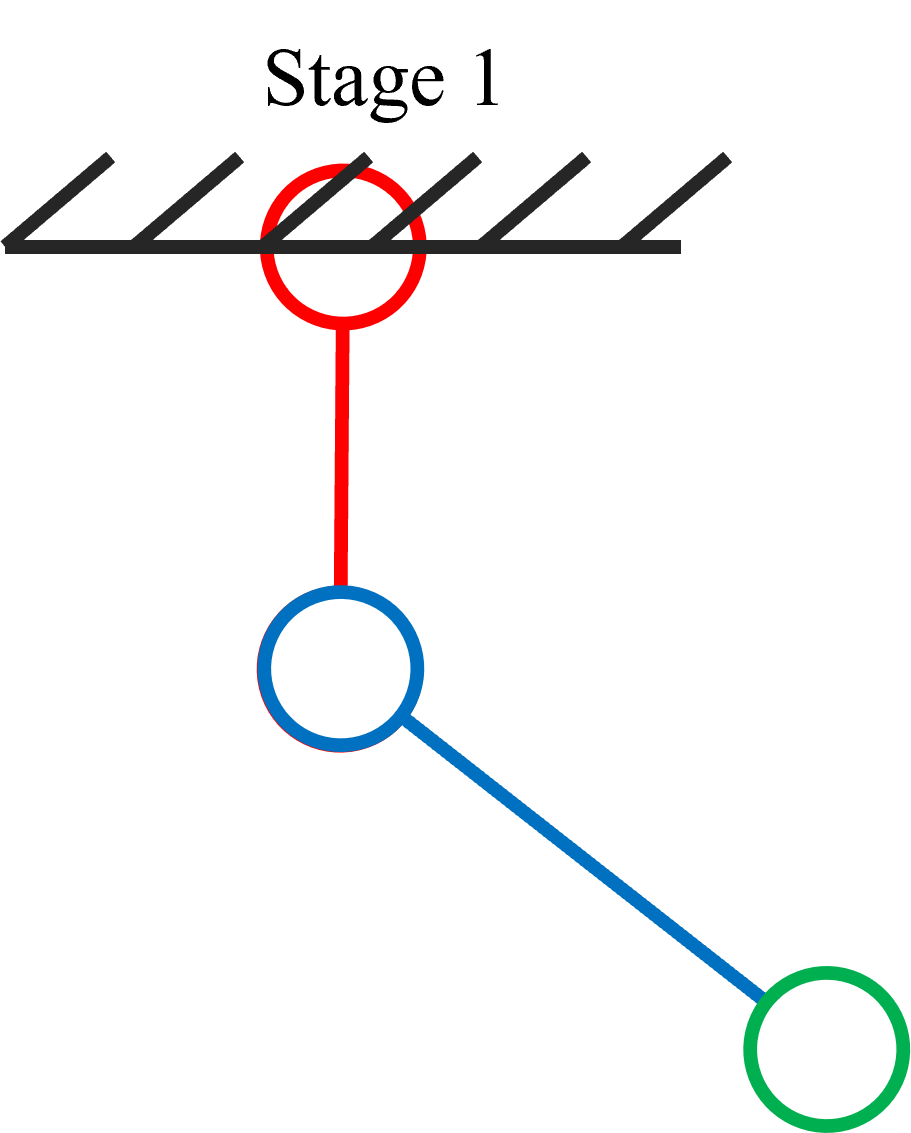
\includegraphics[width=0.25\textwidth]{figures/methodology/stage1.png} % Adjust the width as desired
    \caption{Swing up stage 1}
    \label{fig:my_image_label} % Optional label for referencing
\end{figure}

As the end effector reaches a threshold line \(h_{line} = 0.8(l_1+l_2)\), we
introduce a second level of reward \(r_{line}\). The end effector height is
given by
\begin{align}
    h(p_1, p_2) = -l_1\cos(p_1) - l_2 \cos(p_1 + p_2).
\end{align}

with the link lengths $l_1$ and $l_2$.
This reward provides the agent with a fixed value
but is carefully designed to prevent the system from spinning rapidly in either
clockwise or counterclockwise directions. To discourage the agent from
exploiting rewards by spinning at excessive speeds, a significant penalty
\(-r_{vel}\) is implemented for any speed exceeding $v_{thresh}=8\,
\text{rad}/\text{s}$ in absolute value.
This penalty effectively compels the agent to approach the maximum point while
adhering to the predefined speed interval. The speed penalty was only needed for
the acrobot.

\begin{figure}[H]
    \centering
    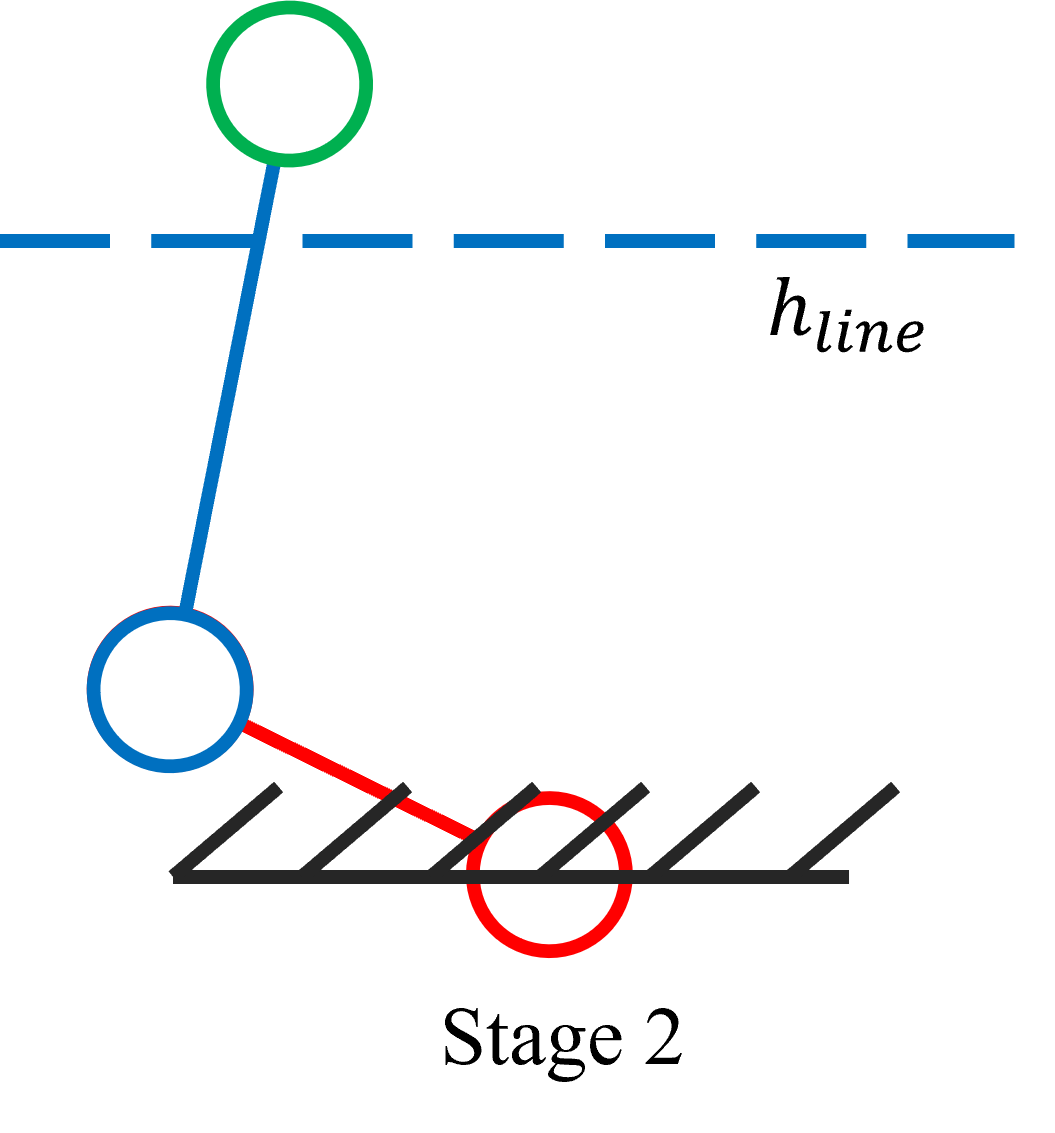
\includegraphics[width=0.25\textwidth]{figures/methodology/stage2.png} % Adjust the width as desired
    \caption{Swing up stage 2}
    \label{fig:my_image_label} % Optional label for referencing
\end{figure}

The third level of reward $r_{LQR}$ aims to provide a substantial reward to the
agent when it remains within the Region of Attraction (RoA) of the LQR
controller. By this we want to achieve that the policy learns to enter the LQR
controller RoA so that there can be a smooth transition between both
controllers. For details on the LQR controller and its region of attraction, we
refer to these lecture notes. The parameters, we used in
the cost matrices of the LQR controller are listed in
Table~\ref{tab:parameters}. We computed the RoA similar to
but with a sums of squares method.  Once the RoA is computed,
it can be checked whether a state $x$ belongs to the estimated RoA of the LQR
controller by calculating the cost-to-go of the LQR controller with the matrix
$S_{LQR}$ and comparing it with the scalar $\rho$.

\begin{figure}[H]
    \centering
    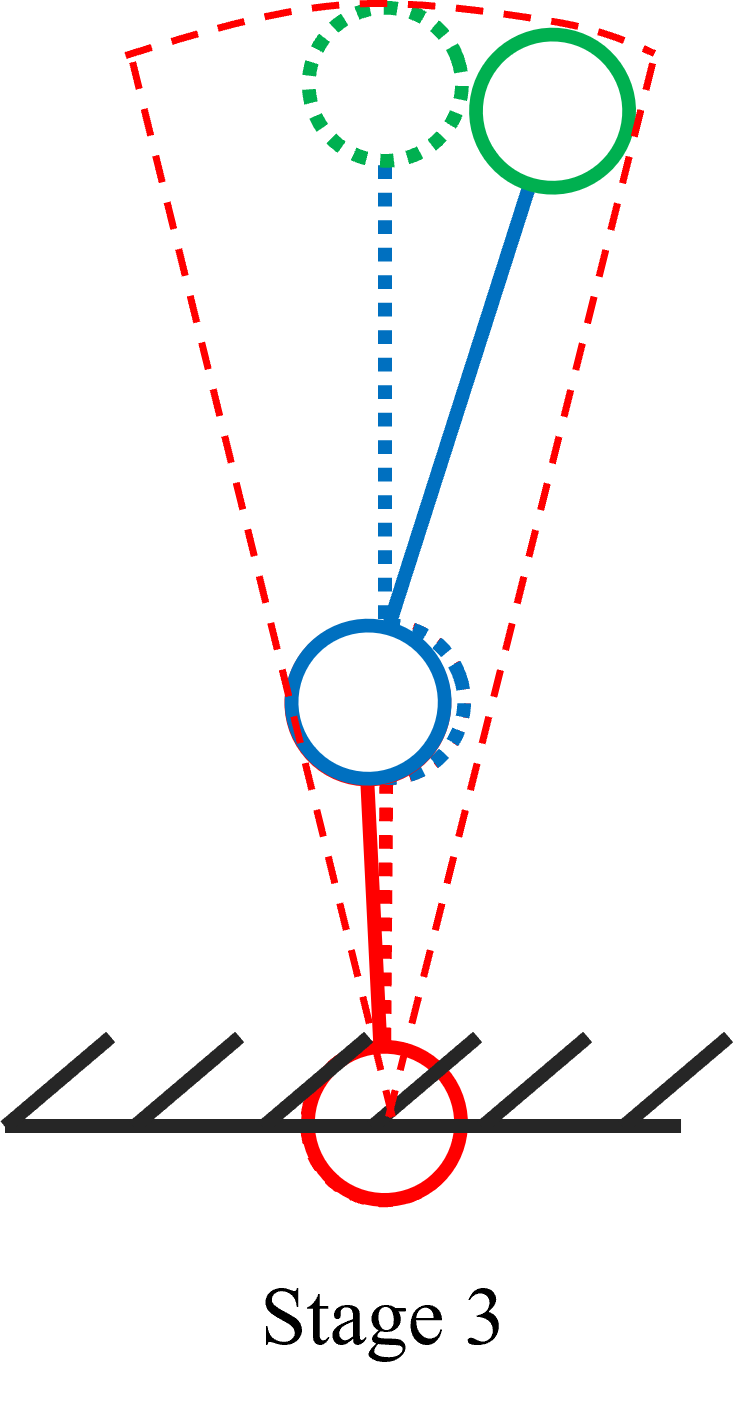
\includegraphics[width=0.25\textwidth]{figures/methodology/stage3.png} % Adjust the width as desired
    \caption{Swing up stage 3}
    \label{fig:my_image_label} % Optional label for referencing
\end{figure}

\cleardoublepage
